\section{Introduction}

\begin{figure}[H]
    \centering
    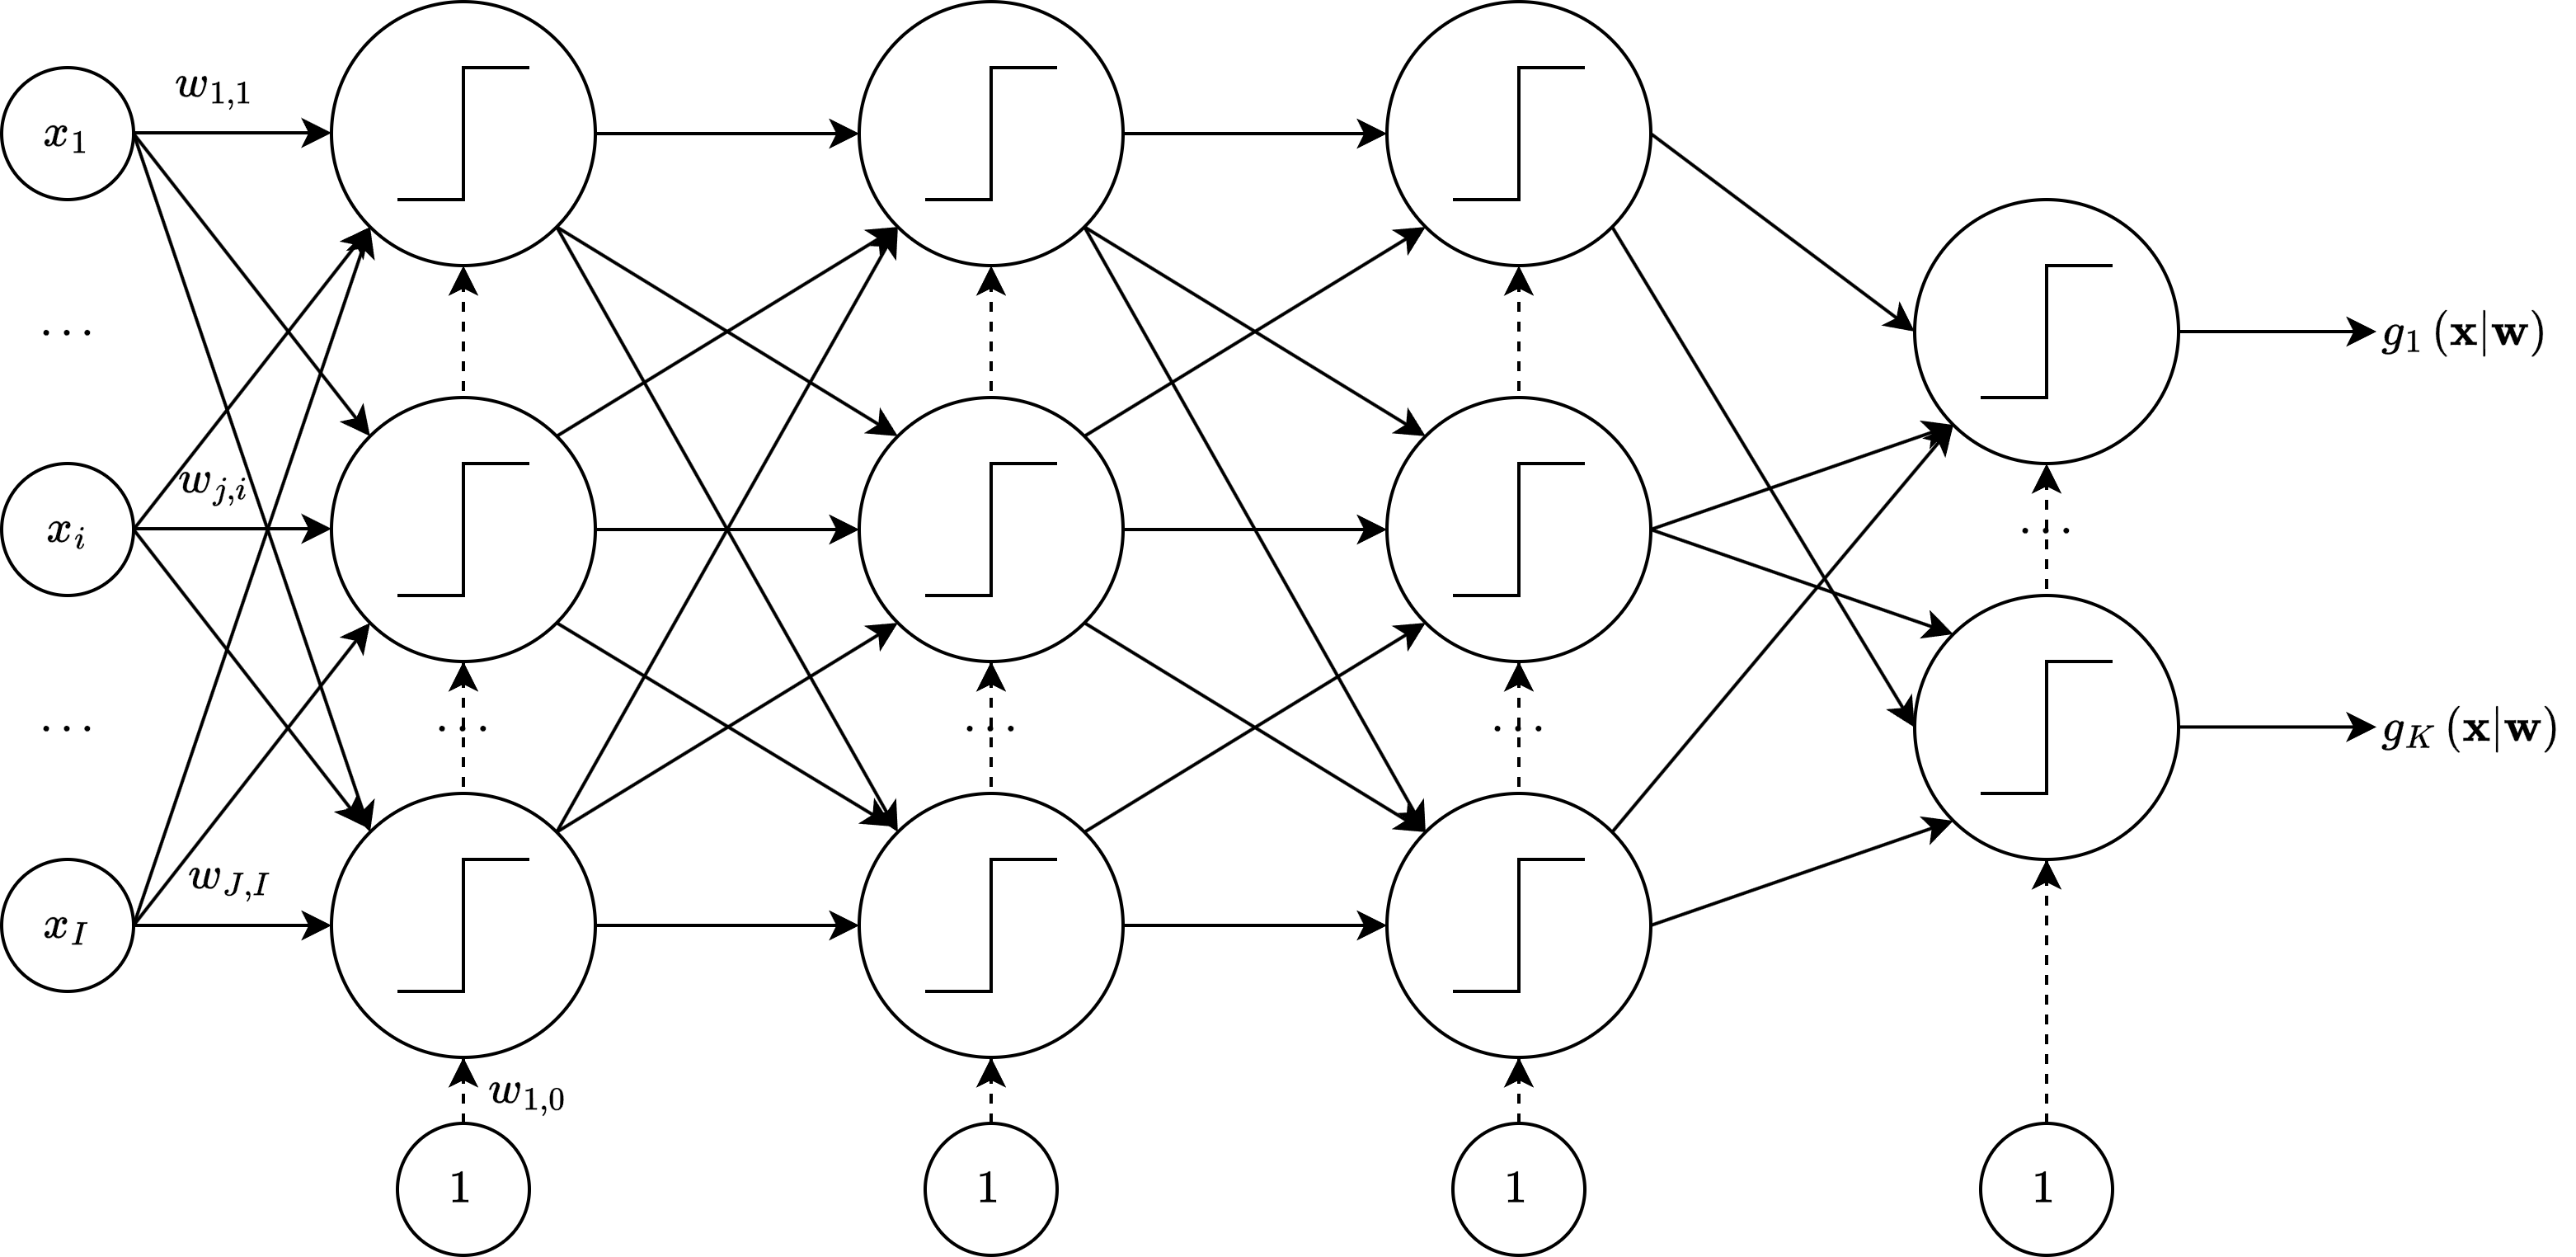
\includegraphics[width=0.75\linewidth]{images/ffnn.png}
    \caption{Multi-Layer Perceptron}
\end{figure}
The MLP si composed by multiple layers:
\begin{itemize}
    \item \textit{Input layer}: takes the input and propagates it to the following layer.
        Its size is dependent on the problem.
    \item \textit{Hidden layers}: in these layers we have the effecive computations. 
        The number of layers and neurons per hidden layer is dependent on a hyyperparameter tuning performed by trials-and-errors. 
    \item \textit{Output layer}: returns the output of the neural network.
        Its size is dependent on the problem.
\end{itemize}
This model is non-linear and it is characterized by the number of neurons, activation functions, and the value of the weights. 
Layers are connected through weights $W^{(l)}=\{w_{ij}^{(l)}\}$. 
Consider $J$ nodes for a layer with $I$ inputs, we have that the the matrix that represents each layer has a dimension of $J \times (I+1)$. 
The output of a neuron depends solely on the previous layer. 
The weights in FFNN can be computed by using a tecnique called backpropagation.